\documentclass[12pt,a4paper]{article}
\usepackage[utf8]{inputenc}
\usepackage[spanish]{babel}
\usepackage{listings}
\usepackage{xcolor}
\usepackage{graphicx}
\usepackage{float}
\usepackage{geometry}
\usepackage{fancyhdr}

\geometry{left=2.5cm,right=2.5cm,top=2.5cm,bottom=2.5cm}

\lstset{
    language={[x86masm]Assembler},
    basicstyle=\footnotesize\ttfamily,
    keywordstyle=\color{blue}\bfseries,
    commentstyle=\color{green!50!black},
    stringstyle=\color{red},
    numbers=left,
    numberstyle=\tiny,
    stepnumber=1,
    frame=single,
    breaklines=true,
    tabsize=4,
    captionpos=b,
    literate={á}{{\'a}}1 {é}{{\'e}}1 {í}{{\'i}}1 {ó}{{\'o}}1 {ú}{{\'u}}1 {ñ}{{\~n}}1
}

\pagestyle{fancy}
\fancyhf{}
\fancyfoot[C]{\thepage}

\begin{document}

% =================== PORTADA ===================
\begin{titlepage}
    \centering
    \vspace*{3cm}
    {\Huge \bfseries Gesti\'on de Notas\\[0.5cm]
    en Ensamblador 8086\par}
    \vspace{2cm}
    {\Large Integrantes: Alejandro Obando\par}
    {\Large                               Josue Chango\par}
    {\Large                               Jardel Maza\par}
    \vspace{1cm}
    {\Large Nrc: 202650\par}

    \vspace{2cm}
    {\large \today\par}
    \vfill
\end{titlepage}

% =================== OBJETIVO ===================
\section{Objetivo del Proyecto}

Desarrollar un programa en ensamblador 8086 que permita gestionar las notas de un grupo de estudiantes. El programa debe solicitar la cantidad de estudiantes a las que se les asignara notas, leer las notas individuales (v\'alidas de 00 a 20), calcular el promedio total, la nota m\'as alta y la nota m\'as baja, y finalmente mostrar un resumen con los resultados.

% =================== DESCRIPCIÓN TÉCNICA ===================
\section{Descripci\'on T\'ecnica}

\subsection{Planteamiento del problema}

Se requiere un sistema que permita al usuario ingresar la cantidad de estudiantes (entre 1 y 9) y posteriormente sus notas correspondientes, valide que cada nota est\'e en el rango de 0 a 20, y finalmente calcule y muestre el promedio, la nota m\'as alta y la nota m\'as baja del grupo de estudiantes. Todo esto debe implementarse en ensamblador 8086 con el emulador emu8086.

\subsection{Algoritmo utilizado}

Cabe recalcar que este algoritmo es construido a partir de algoritmos vistos y resueltos en clase.
\newline
El algoritmo sigue los siguientes pasos:

\begin{enumerate}
    \item Solicitar al usuario la cantidad de estudiantes.
    \item Para cada estudiante:
    \begin{enumerate}
        \item Solicitar la nota como dos d\'igitos individuales (decena y unidad).
        \item Validar que la nota est\'e entre 00 y 20.
        \item Si es inv\'alida, mostrar mensaje de error y repetir la solicitud.
    \end{enumerate}
    \item Convertir cada par de d\'igitos a su valor num\'erico multiplicando la decena por 10 y sumando la unidad.
    \item Calcular la suma total de las notas.
    \item Determinar la nota m\'axima y m\'inima mediante comparaciones sucesivas.
    \item Calcular el promedio mediante restas sucesivas (divisi\'on entera).
    \item Mostrar el resumen: promedio, nota m\'as alta y nota m\'as baja.
\end{enumerate}

\subsection{Instrucciones clave del 8086 utilizadas}

\begin{itemize}
    \item \texttt{MOV}: Transferencia de datos entre registros y memoria.
    \item \texttt{CMP}: Comparaci\'on de dos operandos para la toma de decisiones.
    \item \texttt{JMP}, \texttt{JE}, \texttt{JG}, \texttt{JGE}, \texttt{JL}, \texttt{JNE}: Saltos condicionales e incondicionales para el control de flujo.
    \item \texttt{INT 21h}: Llamadas al sistema operativo para entrada/salida.
    \item \texttt{ADD}, \texttt{SUB}, \texttt{DEC}, \texttt{INC}: Operaciones aritm\'eticas.
    \item \texttt{LEA}: Carga de direcciones efectivas para el manejo de cadenas.
\end{itemize}

% =================== IMPLEMENTACIÓN ===================
\section{Implementaci\'on}

\subsection{Herramientas utilizadas}

\begin{itemize}
    \item \textbf{emu8086} --- Emulador y ensamblador para microprocesadores 8086.
    \item Editor de texto para la escritura del c\'odigo fuente y respectivo informe.
\end{itemize}

\subsection{C\'odigo fuente}

A continuaci\'on se presenta el c\'odigo completo del programa con comentarios explicativos:

\lstinputlisting[language={[x86masm]Assembler}]{Gestion de notas.asm}

% =================== PRUEBAS Y RESULTADOS ===================
\section{Pruebas y Resultados}

\subsection{Casos de prueba}

\begin{table}[h]
\centering
\begin{tabular}{|c|c|c|c|c|}
\hline
\textbf{Caso} & \textbf{Cant. estudiantes} & \textbf{Notas} & \textbf{Promedio esperado} & \textbf{Max/Min esperados} \\ \hline
1 & 3 & 15, 18, 20 & 17 & 20 / 15 \\ \hline
2 & 4 & 10, 12, 14, 16 & 13 & 16 / 10 \\ \hline
3 & 5 & 20, 20, 20, 20, 20 & 20 & 20 / 20 \\ \hline
4 & 2 & 05, 00 & 2 & 05 / 00 \\ \hline
5 & 3 & 07, 11, 14 & 10 & 14 / 07 \\ \hline
\end{tabular}
\caption{Casos de prueba del programa.}
\end{table}

\subsection{Ejecuci\'on del programa}

A continuaci\'on se presentan las capturas de pantalla de cada caso de prueba ejecutado en emu8086:

\begin{figure}[H]
    \centering
    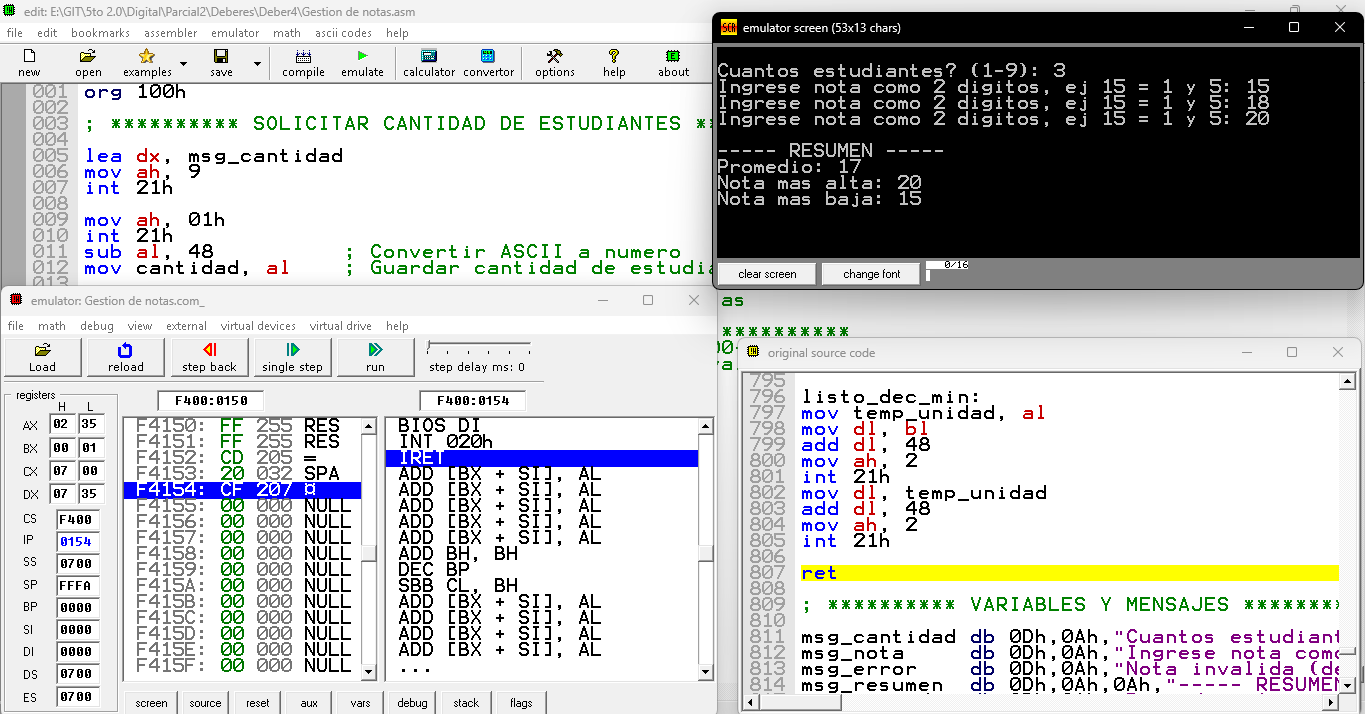
\includegraphics[width=0.8\textwidth]{Caso1.png}
    \caption{Caso 1: 3 estudiantes con notas 15, 18, 20. Promedio esperado: 17, Max: 20, Min: 15.}
\end{figure}

\begin{figure}[H]
    \centering
    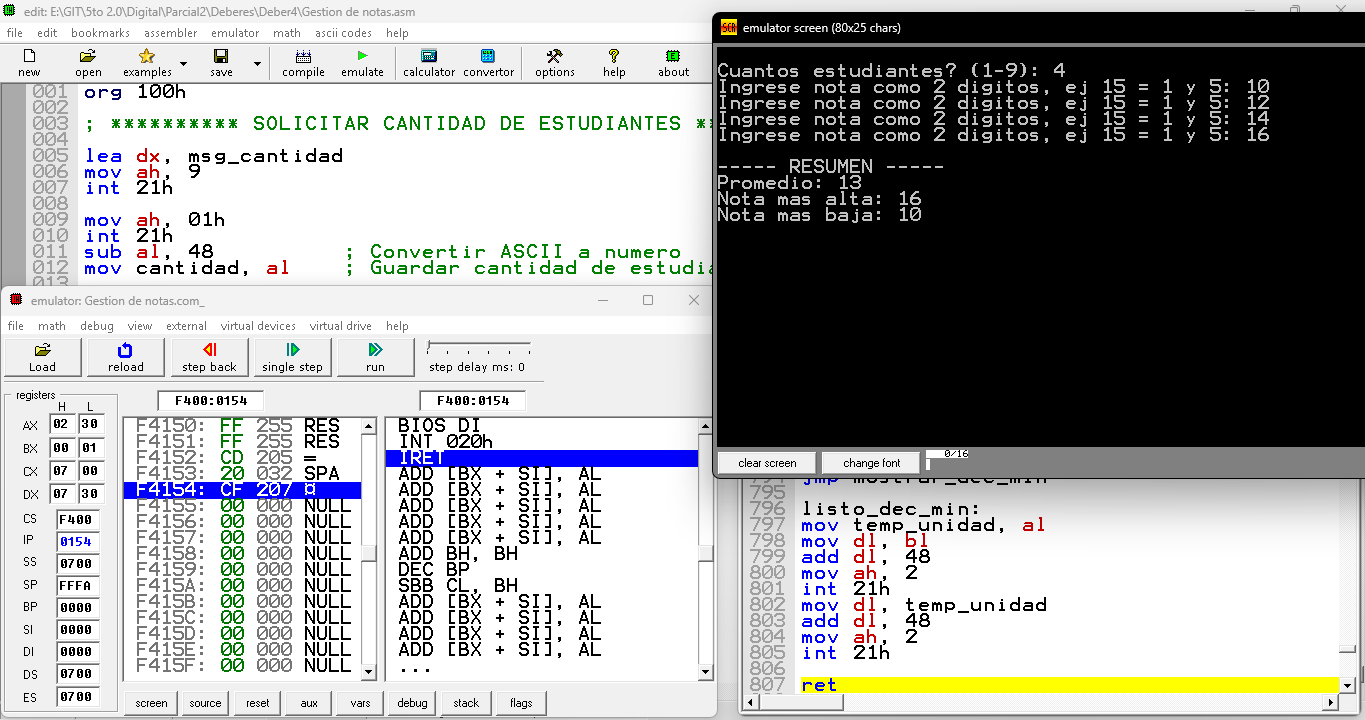
\includegraphics[width=0.8\textwidth]{Caso2.png}
    \caption{Caso 2: 4 estudiantes con notas 10, 12, 14, 16. Promedio esperado: 13, Max: 16, Min: 10.}
\end{figure}

\begin{figure}[H]
    \centering
    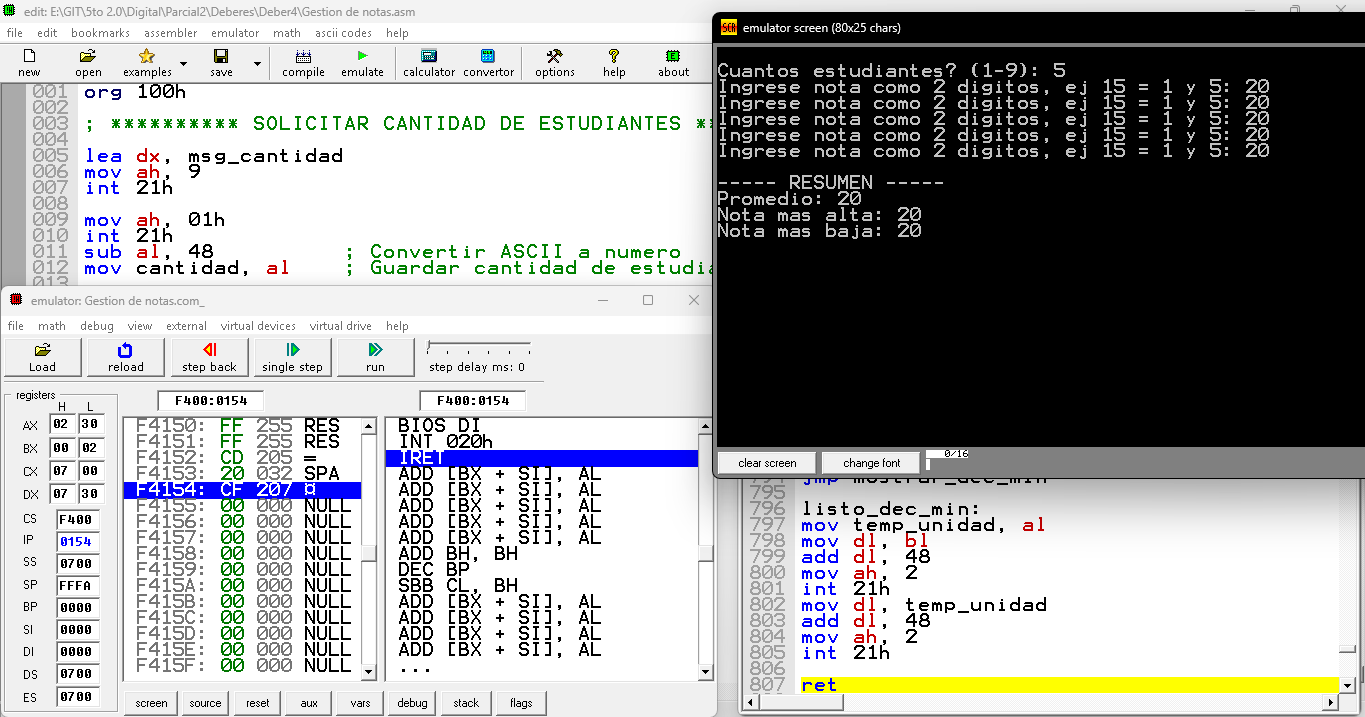
\includegraphics[width=0.8\textwidth]{Caso3.png}
    \caption{Caso 3: 5 estudiantes con notas 20, 20, 20, 20, 20. Promedio esperado: 20, Max: 20, Min: 20.}
\end{figure}

\begin{figure}[H]
    \centering
    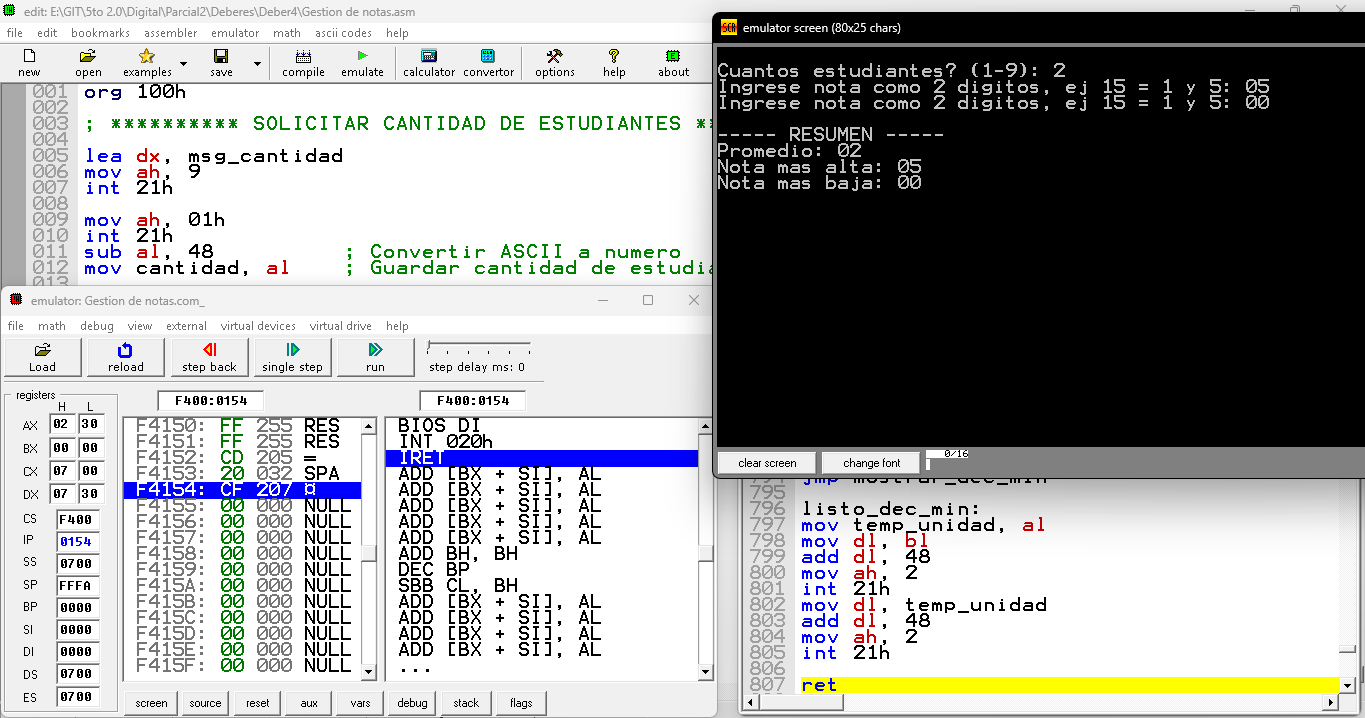
\includegraphics[width=0.8\textwidth]{Caso4.png}
    \caption{Caso 4: 2 estudiantes con notas 05, 00. Promedio esperado: 2, Max: 05, Min: 00.}
\end{figure}

\begin{figure}[H]
    \centering
    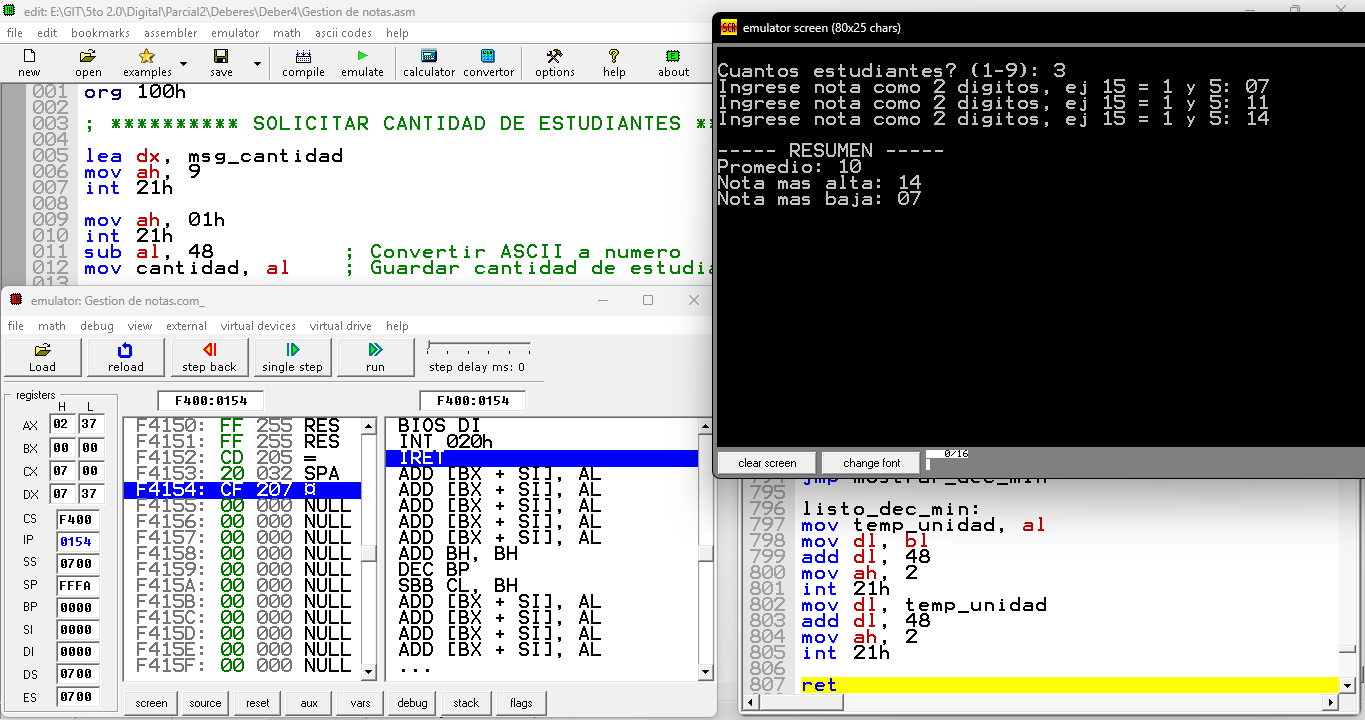
\includegraphics[width=0.8\textwidth]{Caso5.png}
    \caption{Caso 5: 3 estudiantes con notas 07, 11, 14. Promedio esperado: 10, Max: 14, Min: 07.}
\end{figure}

\subsection{Comparaci\'on de resultados}

\begin{table}[H]
\centering
\small
\renewcommand{\arraystretch}{1.2}
\setlength{\tabcolsep}{4pt}
\begin{tabular}{|c|c|c|c|c|c|}
\hline
\textbf{Caso} & \textbf{Notas} & \textbf{Prm. esper.} & \textbf{Prm. obt.} & \textbf{Max/Min esper.} & \textbf{Max/Min obt.} \\ \hline
1 & 15, 18, 20 & 17 & 17 & 20 / 15 & 20 / 15 \\ \hline
2 & 10, 12, 14, 16 & 13 & 13 & 16 / 10 & 16 / 10 \\ \hline
3 & 20, 20, 20, 20, 20 & 20 & 20 & 20 / 20 & 20 / 20 \\ \hline
4 & 05, 00 & 2 & 2 & 05 / 00 & 05 / 00 \\ \hline
5 & 07, 11, 14 & 10 & 10 & 14 / 07 & 14 / 07 \\ \hline
\end{tabular}
\caption{Comparaci\'on entre resultados esperados y obtenidos.}
\end{table}

Como se observa en la tabla, todos los resultados obtenidos coinciden exactamente con los que se esperan, lo que demuestra que el programa funciona de manera correcta.

% =================== CONCLUSIONES ===================
\section*{Conclusiones}
\addcontentsline{toc}{section}{Conclusiones}

El programa desarrollado cumple con el objetivo de gestionar notas mediante ensamblador 8086, ya que permite ingresar hasta 10 notas, tambi\'en valida que cada una est\'e en el rango permitido (00--20), y calcula correctamente el promedio, asi mismo se observan tanto la nota m\'as alta como la nota m\'as baja.

La implementaci\'on con instrucciones b\'asicas del 8086 como \texttt{MOV}, \texttt{CMP}, \texttt{ADD} y saltos condicionales demuestra que con el emulador se puede crear varios programas sencillos pero a la vez funcionales haciendo uso del lenguaje ensamblador para resolver problemas de l\'ogica.

Se puede concluir que el programa es funcional, confiable y cumple con todos los requisitos planteados en el objetivo del proyecto.

\end{document}
